\documentclass[a4paper]{article}
\usepackage[margin = 1 in]{geometry}
\usepackage{fancyhdr}
\usepackage{lastpage}
\usepackage{ctex}
\usepackage[utf8]{inputenc} % Required for inputting international characters
\usepackage[T1]{fontenc} % Output font encoding for international characters
\usepackage[sfdefault]{ClearSans} % Use the Clear Sans font (sans serif)
\usepackage{tocloft} 
\usepackage[hidelinks]{hyperref}
\usepackage{makecell}%导入表格宏包
\usepackage{bmpsize}
\usepackage{graphicx}
\usepackage{epstopdf}
\usepackage{caption}
\usepackage{enumitem}
\usepackage{float}
\usepackage{multirow}
\usepackage{makecell}
\usepackage{amsmath} 
\usepackage{listings}
\usepackage{xcolor}

\author{Vergil/Zijun Li李子骏}
\title{Week 2}
\date{2023.4.10}

\lstset{
  language=Python,
  basicstyle=\ttfamily\small,
  numbers=left,
  numberstyle=\tiny\color{gray},
  stepnumber=1,
  numbersep=5pt,
  backgroundcolor=\color{white},
  showspaces=false,
  showstringspaces=false,
  showtabs=false,
  frame=single,
  rulecolor=\color{black},
  tabsize=4,
  captionpos=b,
  breaklines=true,
  breakatwhitespace=false,
  keywordstyle=\color{blue},
  commentstyle=\color{gray},
  stringstyle=\color{red}
}

\begin{document}
\maketitle
\noindent目前为了评估补贴策略优化效果,希望基于实验数据进行分析,实验组A为优化策略,实验组B为现有策略

\noindent1.	实验分流是否均匀?实验组A人群的转化率和购买人群人均购买金额是否显著高于对照组

\begin{figure}[H]
    \centering
    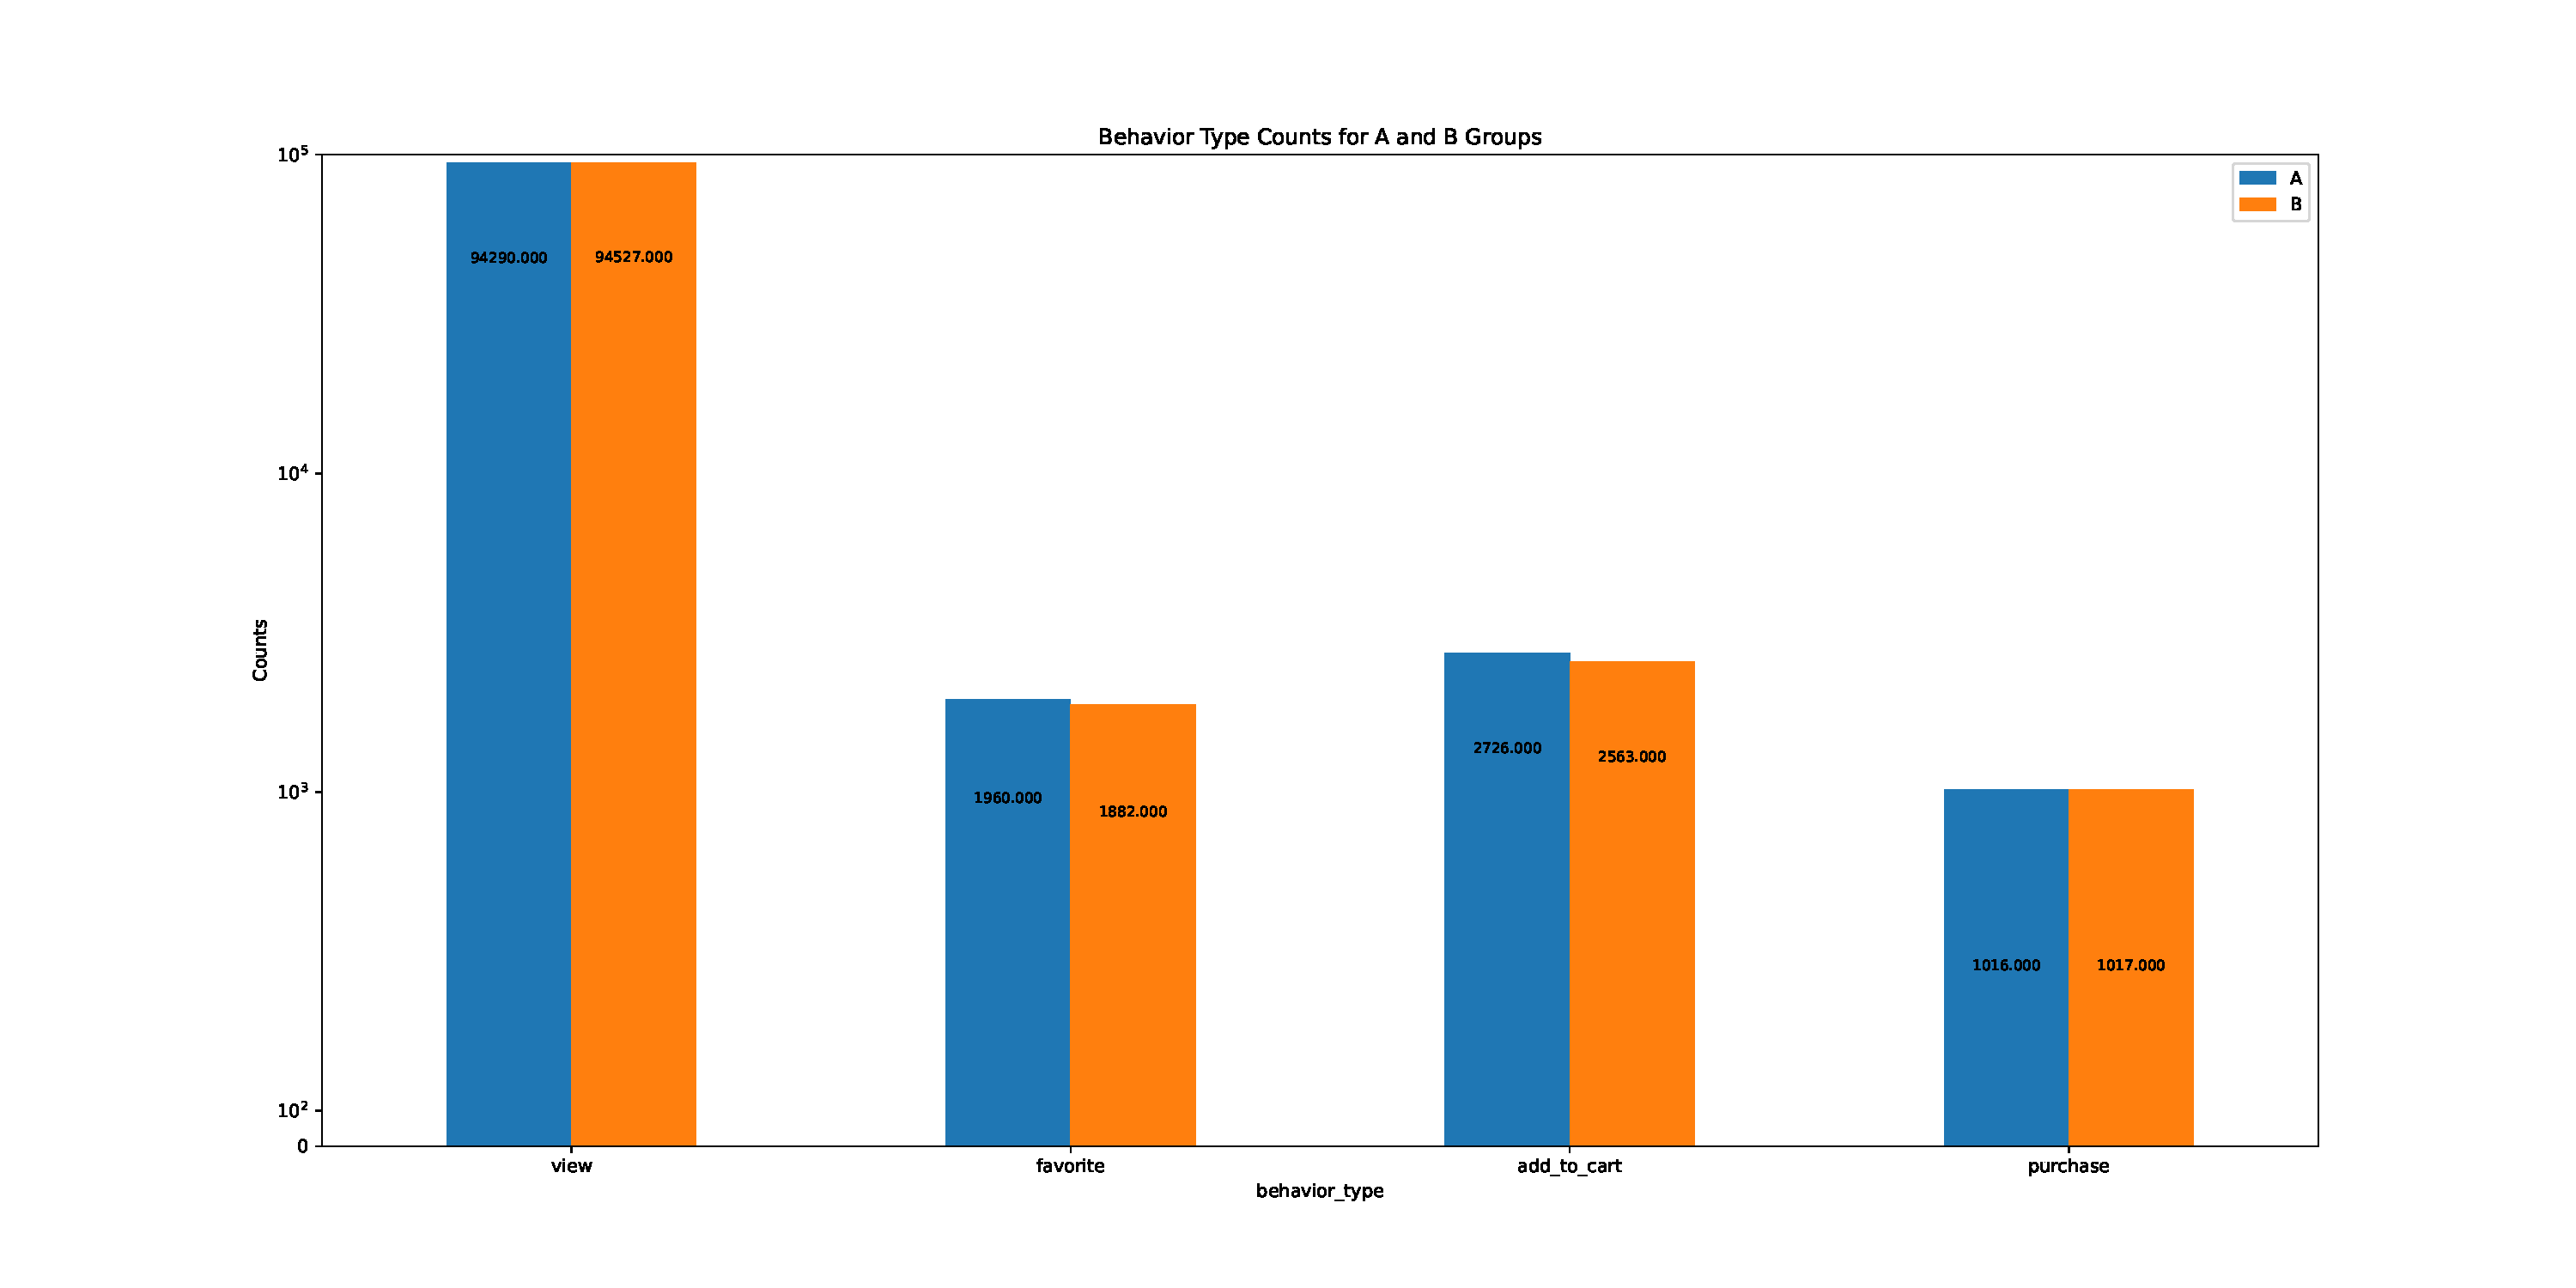
\includegraphics[width=1\textwidth]{./AB_Count.pdf}
    \caption{实验分流均匀对照\_数量}
    \label{fig:experiment1}
\end{figure}

\begin{figure}[H]
	\centering
	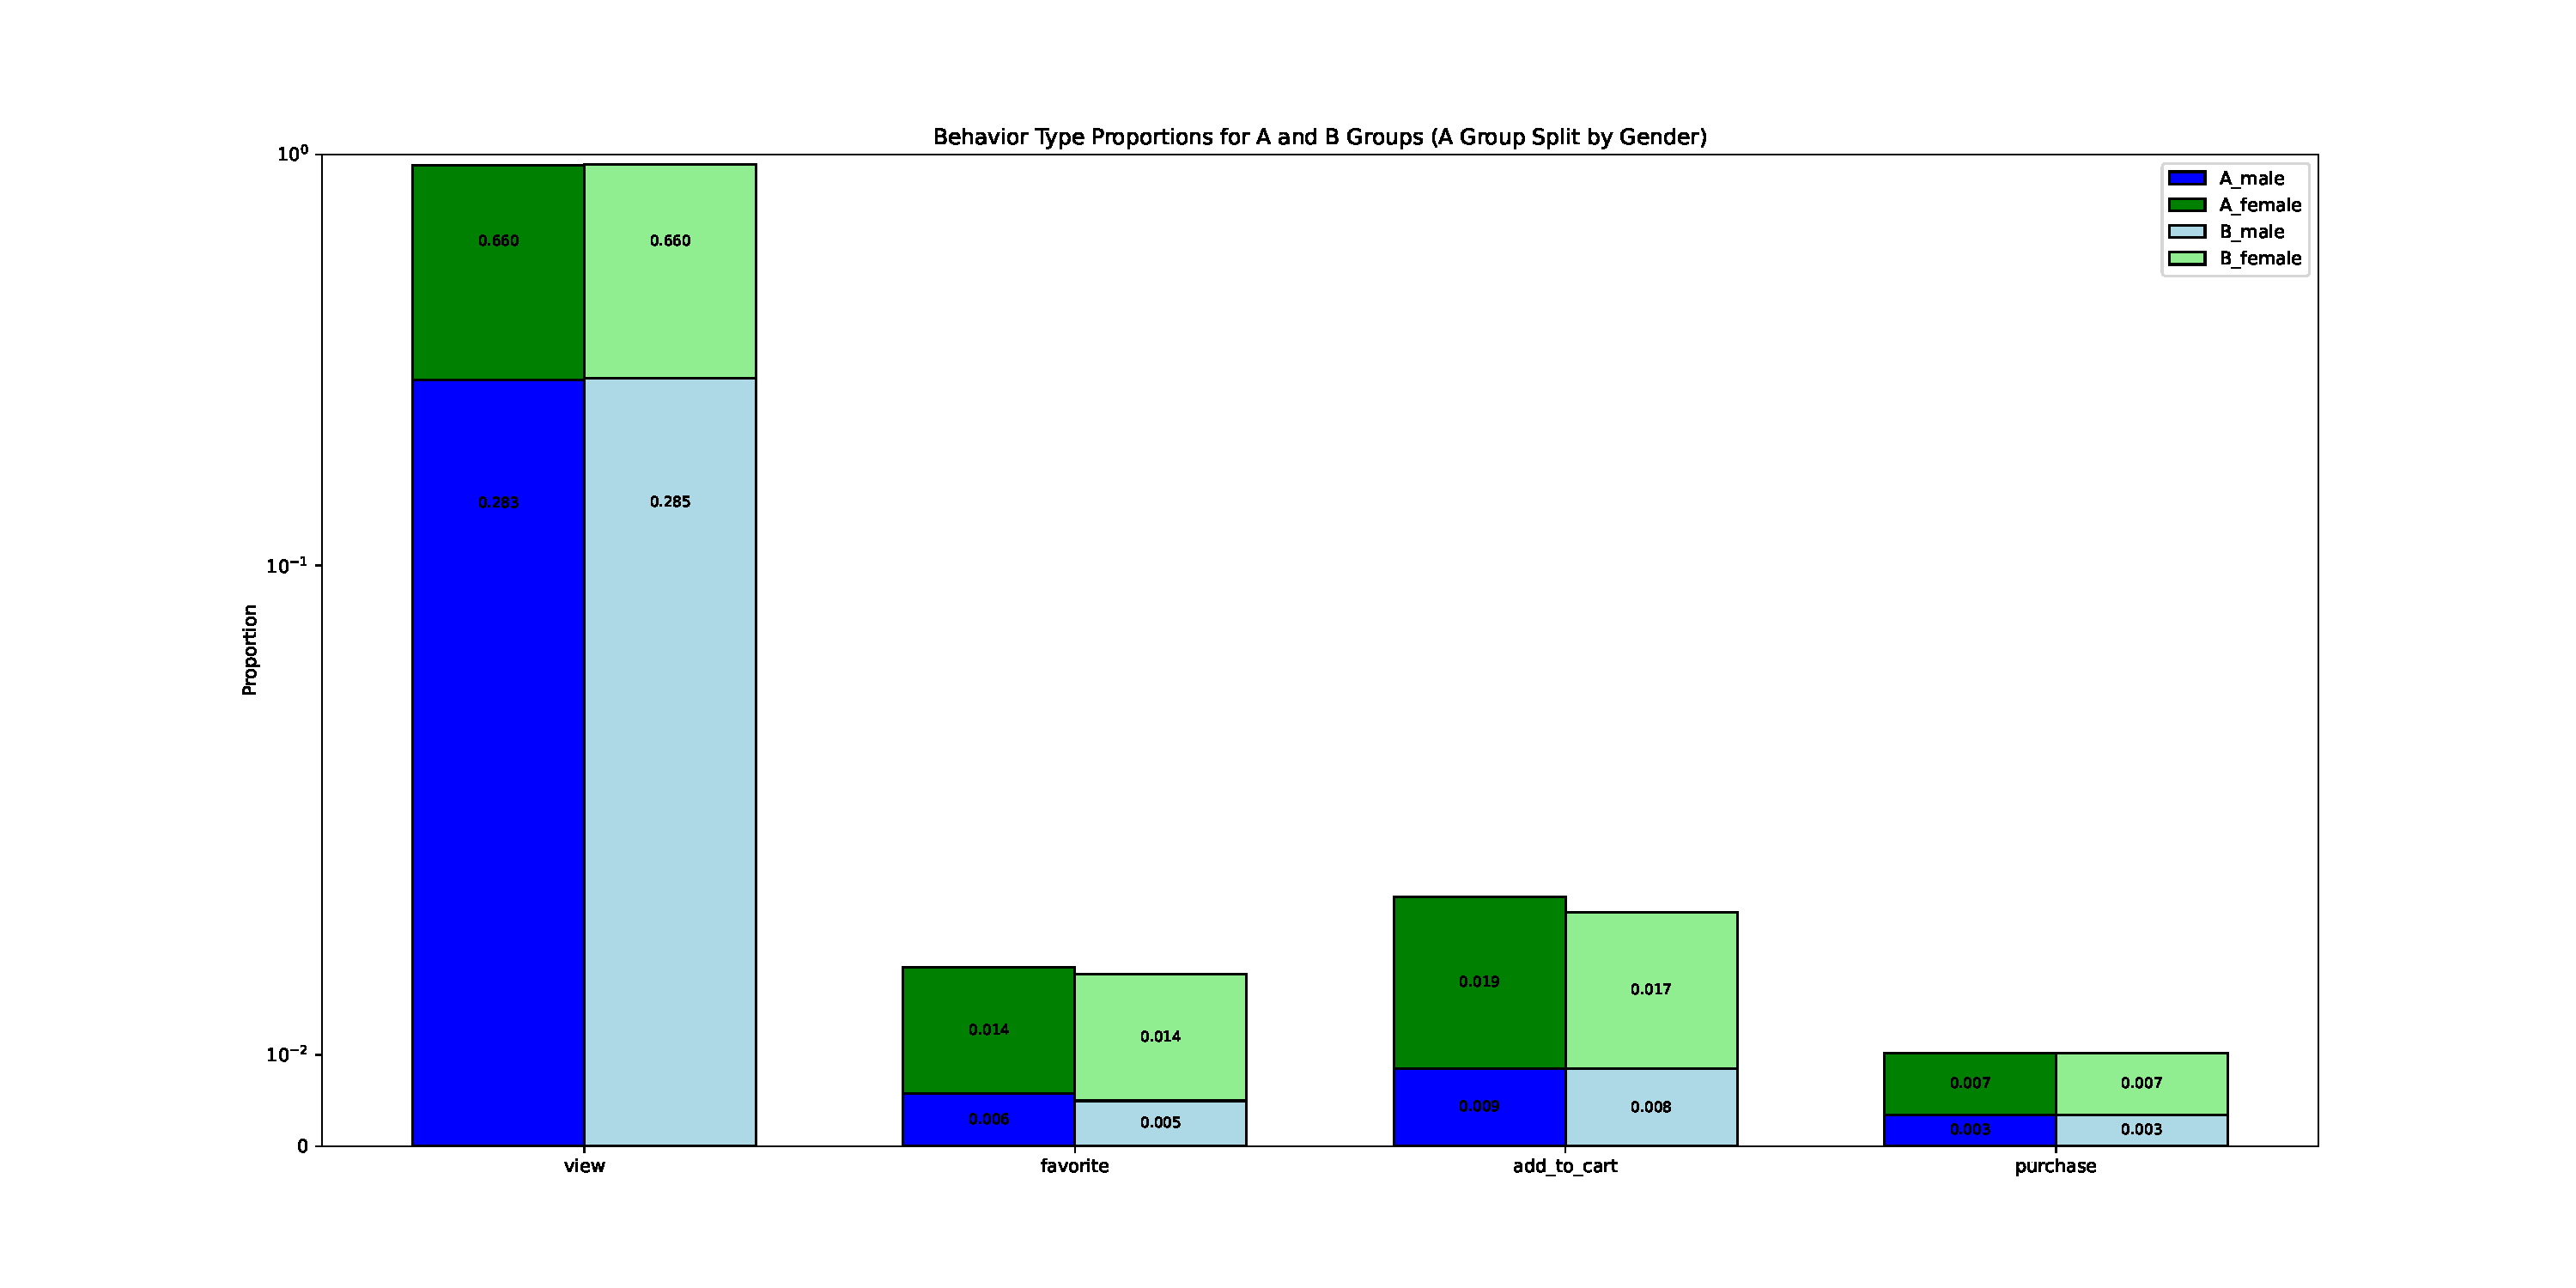
\includegraphics[width=1\textwidth]{./AB_Gender.pdf}
	\caption{实验分流均匀对照\_性别}
	\label{fig:2}
\end{figure}

\begin{figure}[H]
	\centering
	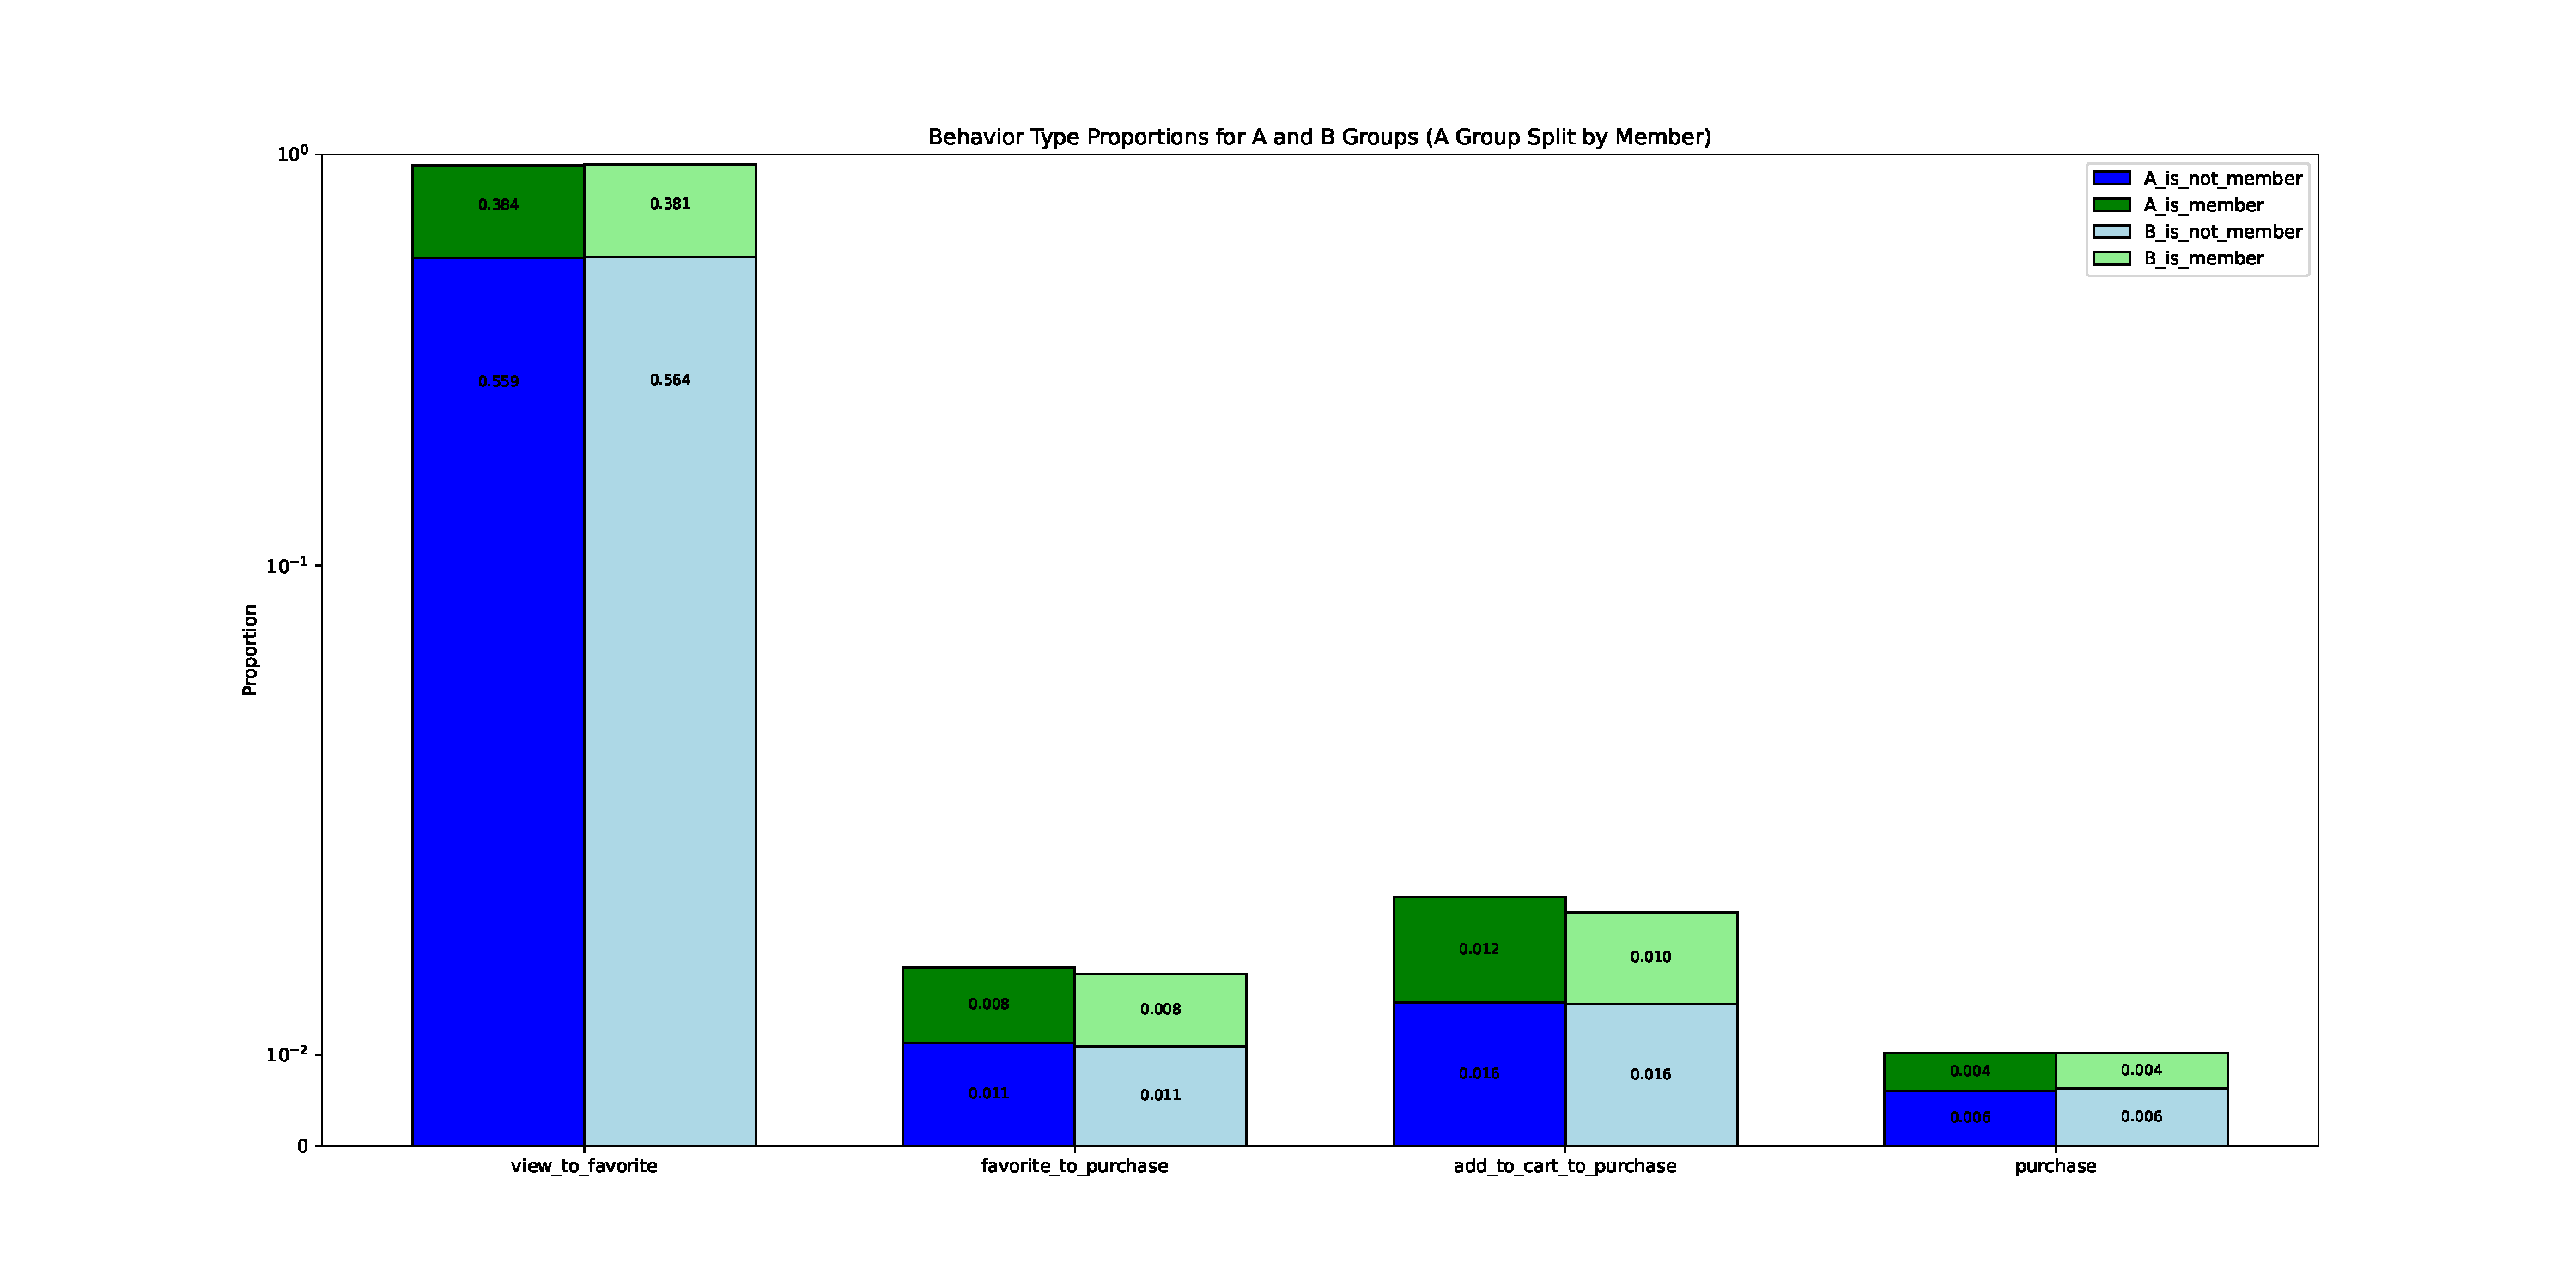
\includegraphics[width=1\textwidth]{./AB_Member.pdf}
	\caption{实验分流均匀对照\_会员}
	\label{fig:3}
\end{figure}

\begin{figure}[H]
	\centering
	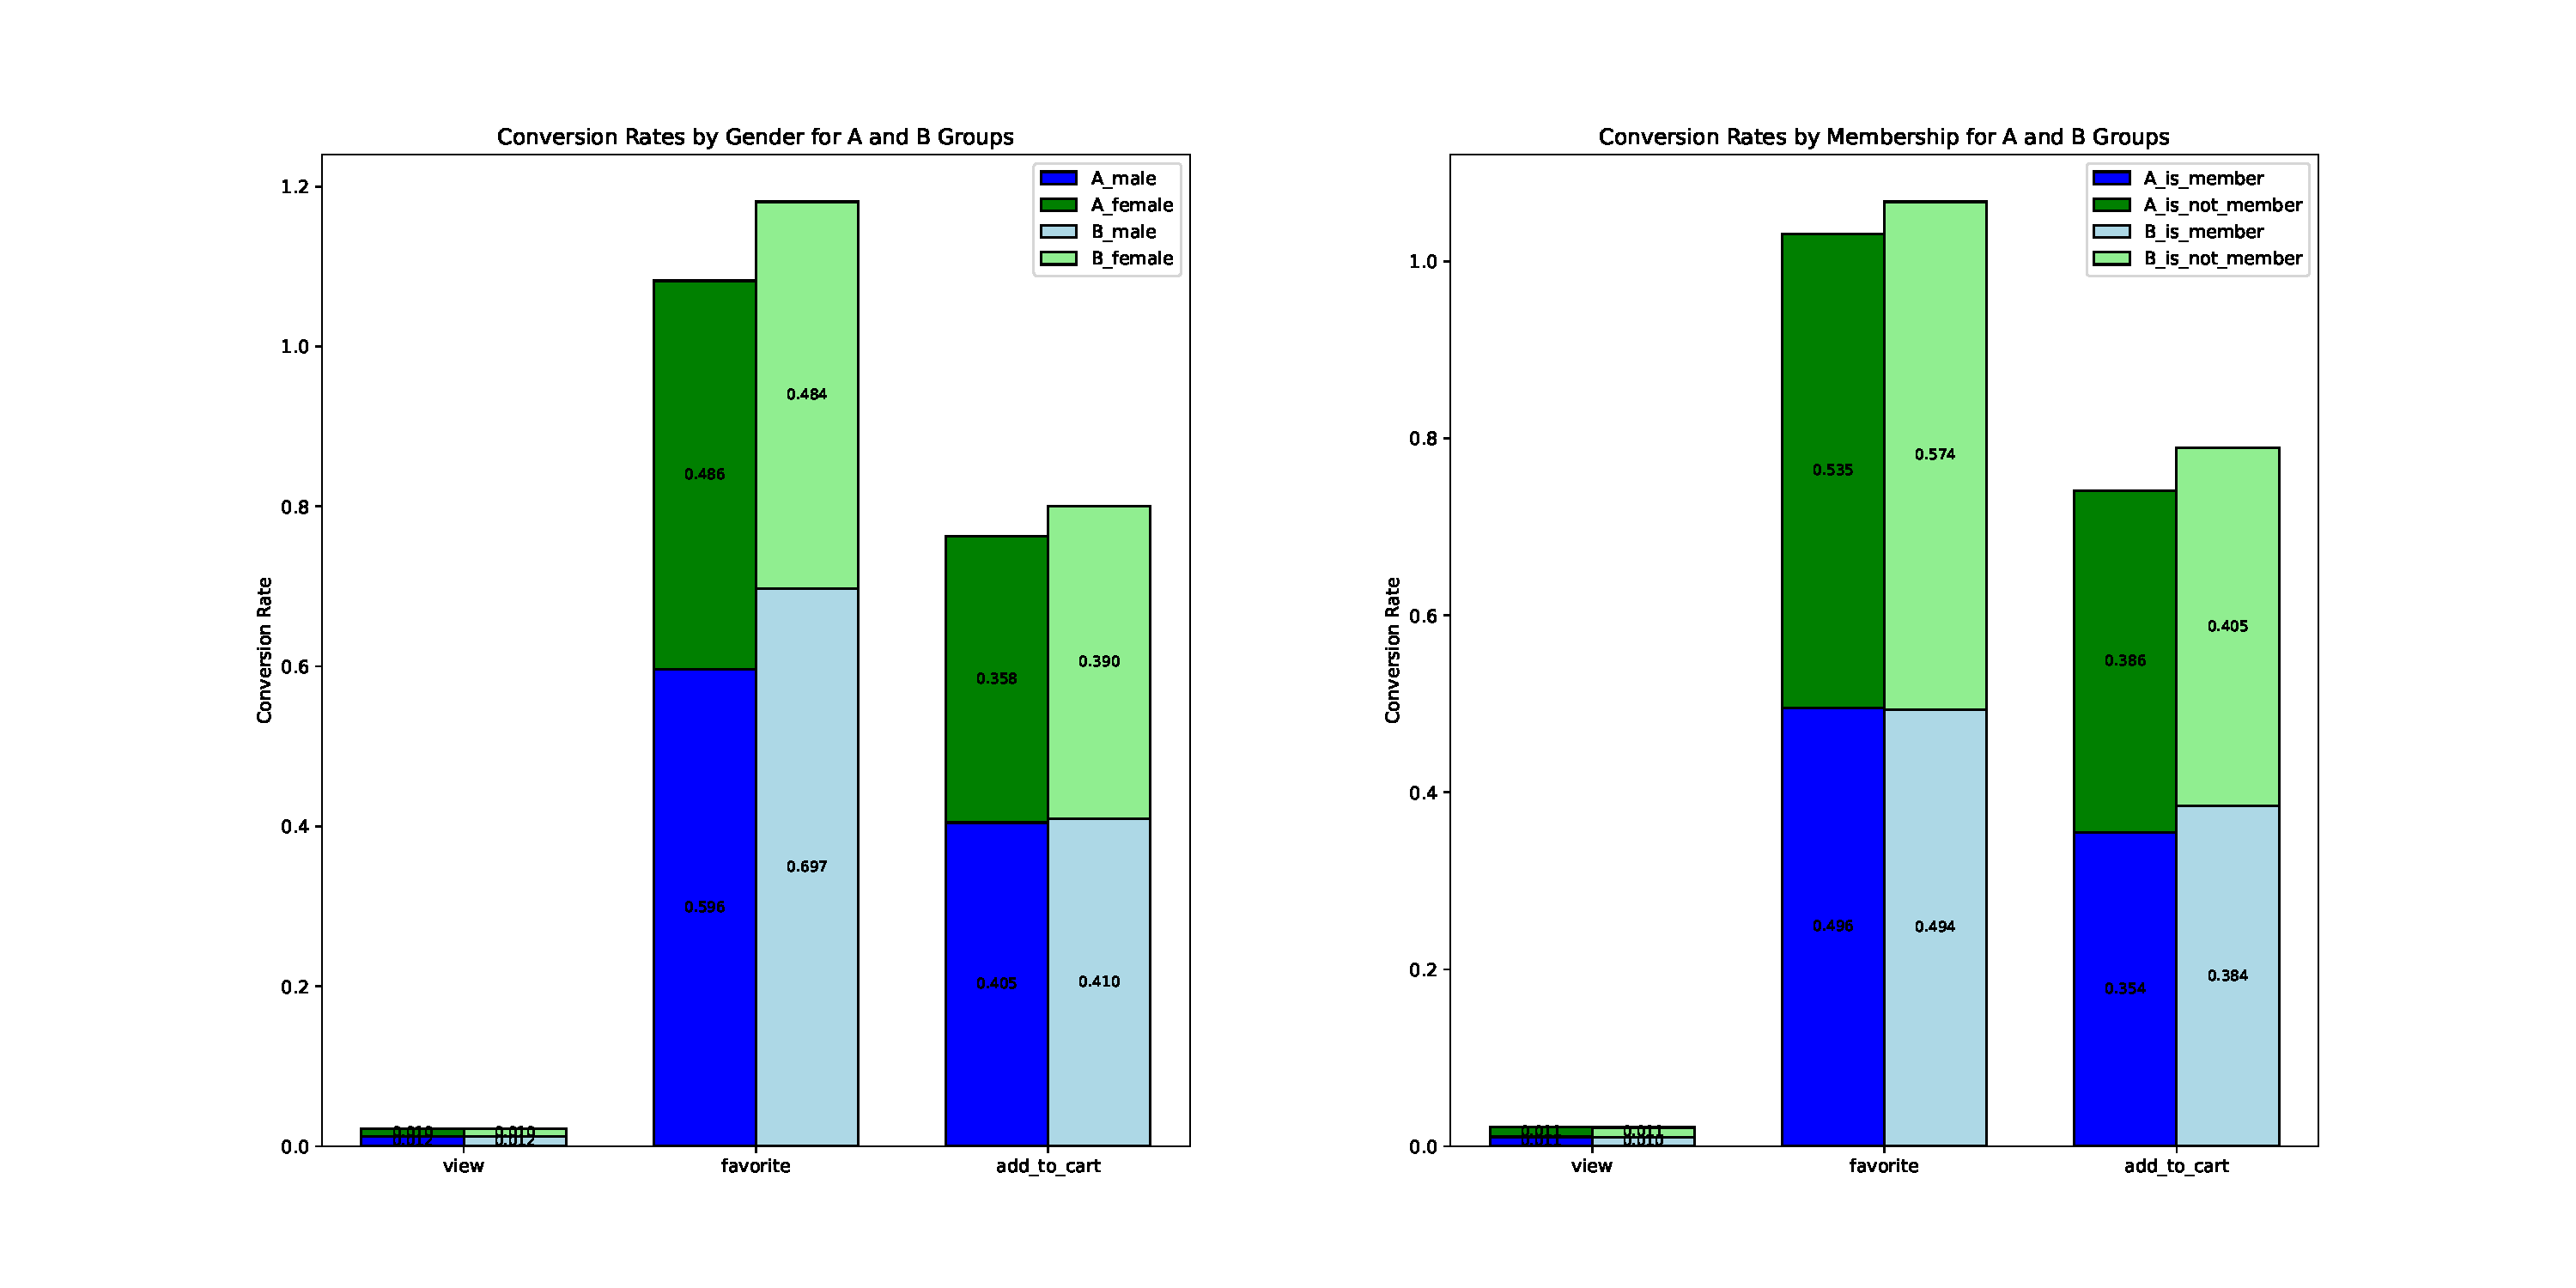
\includegraphics[width=1\textwidth]{./Conversion_rate.pdf}
	\caption{实验分流转化率}
	\label{fig:4}
\end{figure}

\begin{figure}[H]
	\centering
	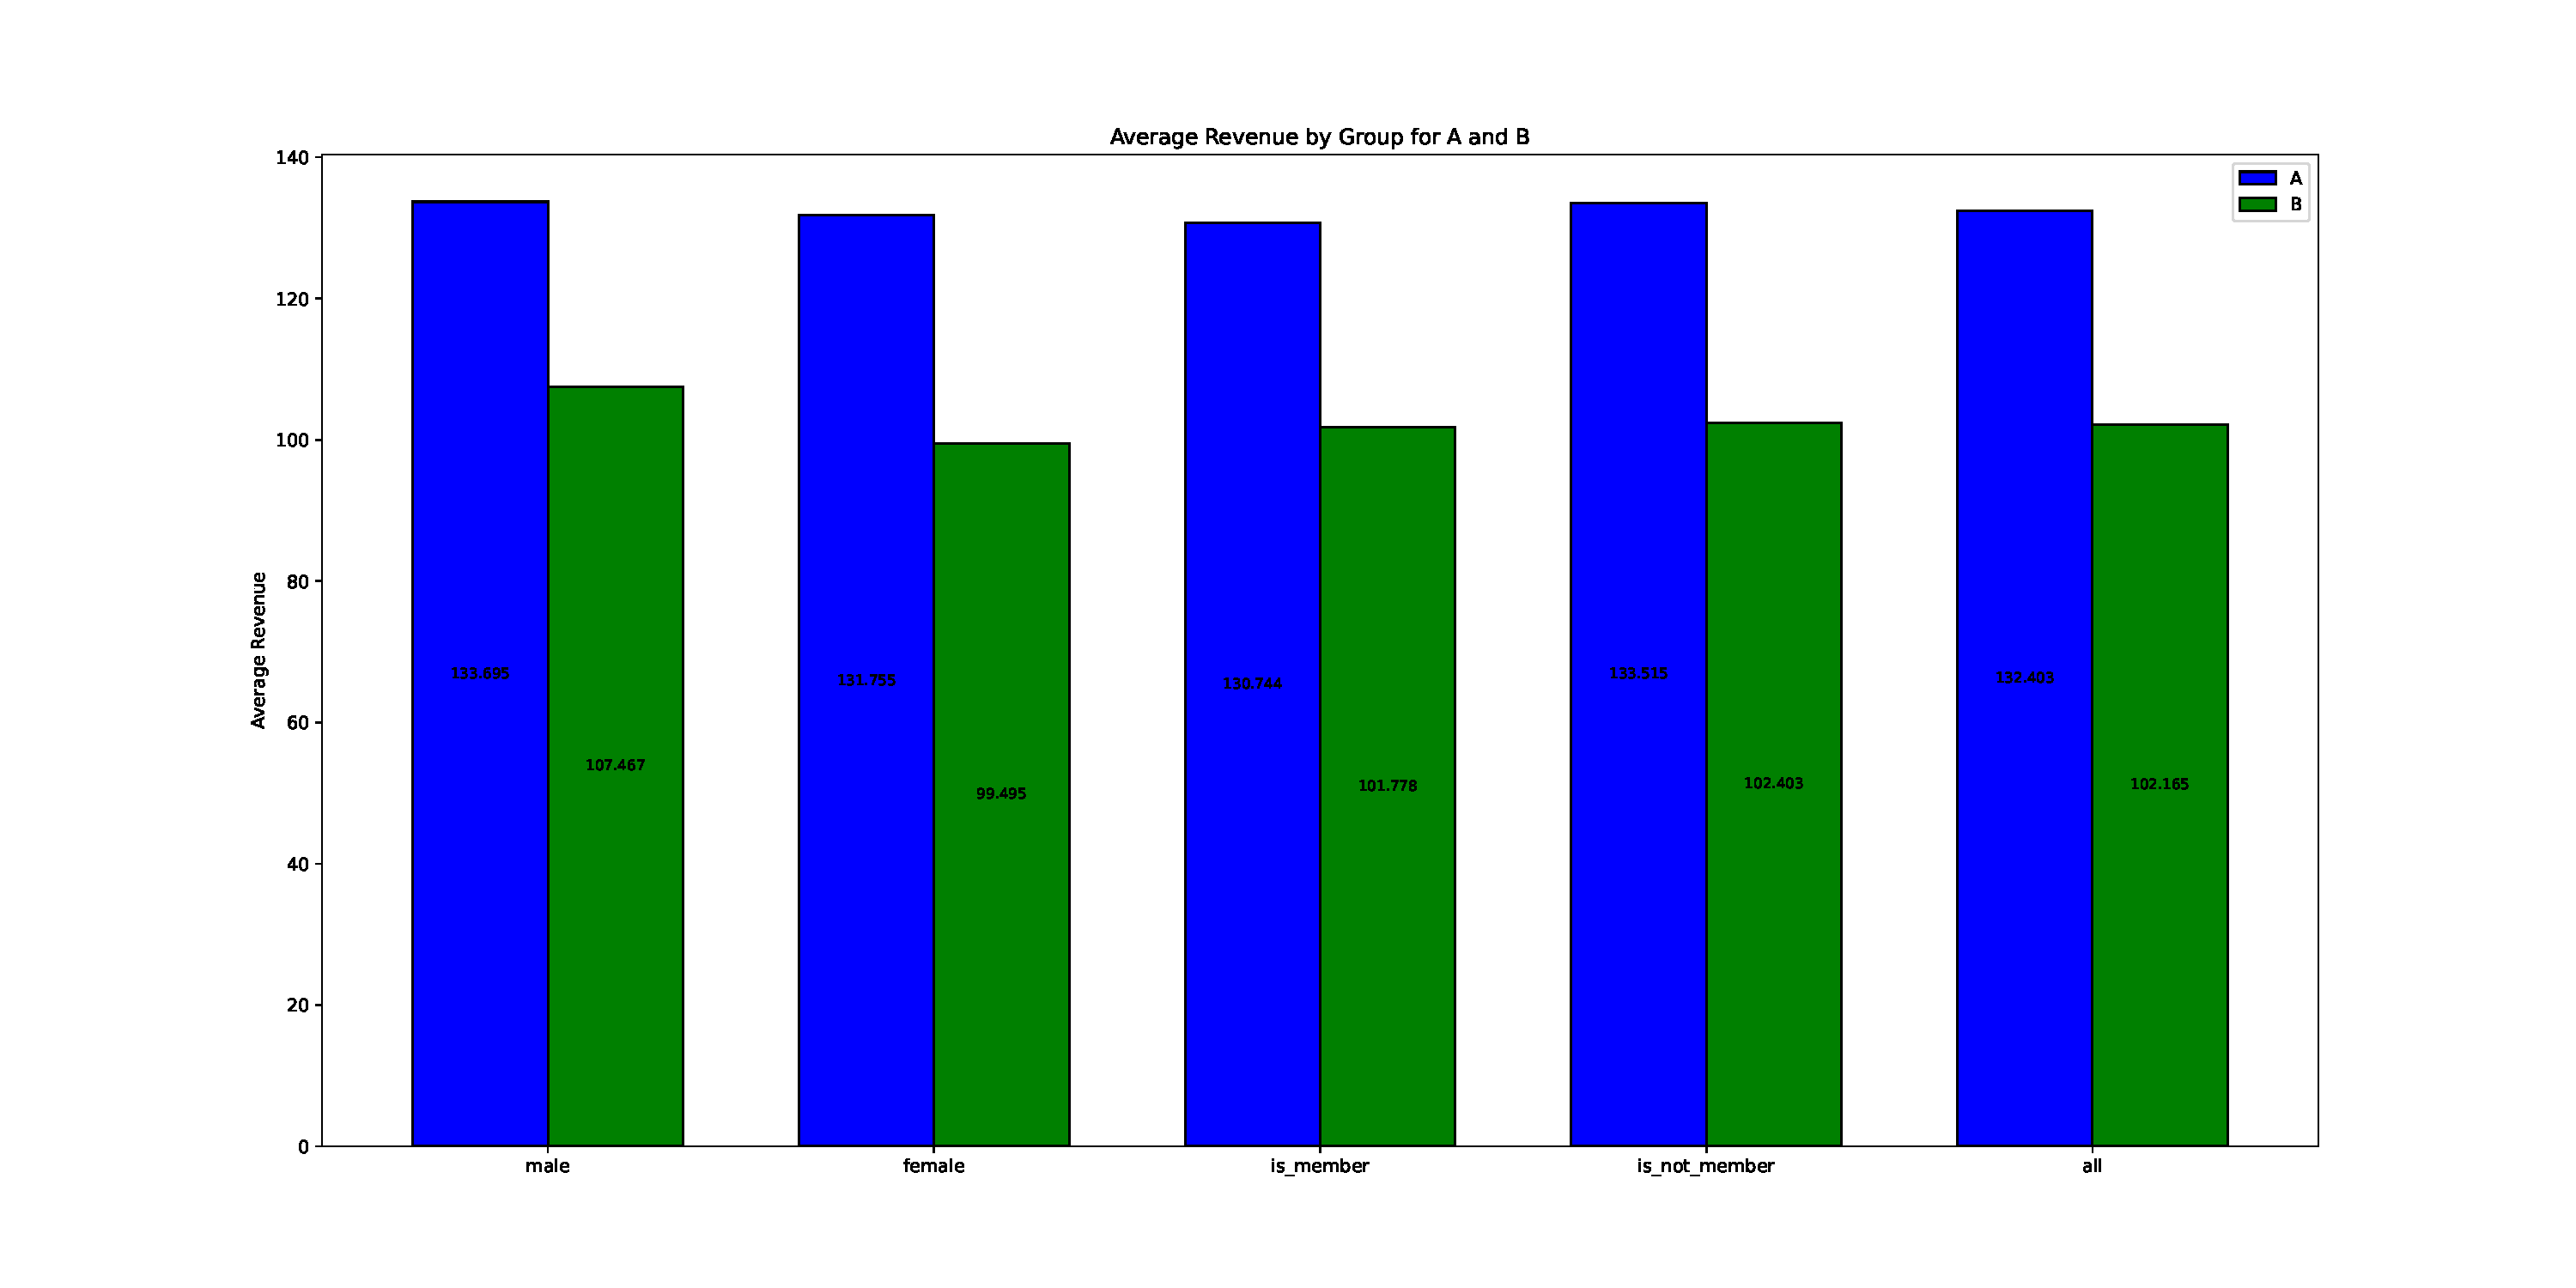
\includegraphics[width=1\textwidth]{./Average_revenue.pdf}
	\caption{实验分流人均金额}
	\label{fig:5}
\end{figure}

\noindent2.	哪类人群在优化策略上提升更为显著?

\begin{lstlisting}[language=Python]
    def revenue_by_group(df, gender=None, is_member=None):
    purchases = df[df['behavior_type'] == 4]
    if gender is not None:
        purchases = purchases[purchases['gender'] == gender]
    if is_member is not None:
        purchases = purchases[purchases['is_member'] == is_member]

    return purchases['revenue']

    print(sw.ztest(revenue_by_group(a_group), revenue_by_group(b_group), value=0))
    print(sw.ztest(revenue_by_group(a_group, gender=0, is_member=0),revenue_by_group(b_group, gender=0, is_member=0) , value=0))
    print(sw.ztest(revenue_by_group(a_group, gender=1, is_member=0),revenue_by_group(b_group, gender=1, is_member=0) , value=0))
    print(sw.ztest(revenue_by_group(a_group, gender=0, is_member=1),revenue_by_group(b_group, gender=0, is_member=1) , value=0))
    print(sw.ztest(revenue_by_group(a_group, gender=1, is_member=1),revenue_by_group(b_group, gender=1, is_member=1) , value=0))

    # (8.951065059372802, 3.520687879890345e-19)
    # (6.293855486513557, 3.0967614748862214e-10)
    # (3.8198188408996328, 0.00013354972484914368)
    # (4.6475147384718865, 3.359580967886752e-06)
    # (2.4626185981981155, 0.013792654878456814)
\end{lstlisting}

第一个结果:(8.951065059372802, 3.520687879890345e-19) 与所有人群进行比较。Z 值较高,P 值远小于 0.05,表示实验组 A 的优化策略对整个人群产生了显著的正效果。

第二个结果:(6.293855486513557, 3.0967614748862214e-10) 与非会员女性进行比较。Z 值较高,P 值远小于 0.05,表示实验组 A 的优化策略对非会员女性产生了显著的正效果。

第三个结果:(3.8198188408996328, 0.00013354972484914368) 与非会员男性进行比较。Z 值适中,P 值远小于 0.05,表示实验组 A 的优化策略对非会员男性产生了显著的正效果。

第四个结果:(4.6475147384718865, 3.359580967886752e-06) 与会员女性进行比较。Z 值较高,P 值远小于 0.05,表示实验组 A 的优化策略对会员女性产生了显著的正效果。

第五个结果:(2.4626185981981155, 0.013792654878456814) 与会员男性进行比较。Z 值适中,P 值略小于 0.05,表示实验组 A 的优化策略对会员男性产生了较为显著的正效果。

对非会员女性, 提升最为明显

\end{document}